\section{The Dynamic Grid}
By now, it is hopefully clear to the reader why dynamic parameters would make an interesting case in the field of physical modelling, and why dynamic grids would be a good solution to undesirable behaviour such as a decrease in bandwidth and increase in numerical dispersion discussed in Section \ref{sec:quality}. %This section will describe the problems that arise when adding and removing grid points. Afterwards, some iterations done over the course of this project and their drawbacks will be shown, leading up to the final implementation of the dynamic grid. 

% The first questions that need to be answered are ``where to add points?" and ``how to add points?" The problems when doing this range from artifacts or auditory `clicks' in the output sound to ``exploding" systems due to artificial injection of energy. 
First, this section will list the requirements of a method that dynamically changes FDTD grid configurations. Then, the iterations done over the course of this project will briefly be described, the details of each can be found in Appendix \ref{app:A}. \SWcomment[(I think I might remove the iterations and appendix actually..)] Finally, the proposed method will be described in detail and summarised in the end.

\subsection{Method requirements}\label{sec:methodReq}
Ideally, a method that dynamically changes the grid size of finite-difference schemes should
\begin{enumerate}
    \item generate an output with a fundamental frequency $f_0$ %described by Eq. \eqref{eq:fundamentalFreq} 
    which is linearly proportional to $c$ ($f_0 \propto c$),
    \item allow for a fractional $N$ to smoothly transition 
    %between different $f_0$s,
    %\item smoothly transition 
    between different grid configurations so that no auditory artefacts are present in the output sound,
    \item generate an output containing harmonic partials -- or modes -- which are integer multiples of the fundamental ($f_p = f_0 p$ with integer $p$),
    \item generate an output with $\lfloor N\rfloor-1$ modes corresponding to the number of moving points of the system ($p = [1, \hdots, \lfloor N\rfloor-1]$),\\
    \item work in real time.
\end{enumerate}
The last requirement is an optional one, but in order for the final implementation to be ``playable'', this is necessary. 
%
% The total amount of modes is expected to be equal to $N-1$ corresponding to the total number of moving grid points (points excluding the boundary).
%As the variables $c$, $h$, $\lambda$ and $N$ are now time-varying, a superscript $n$ or $n-1$ is added when necessary. If omitted, a time index $n$ is assumed.

\subsection{Iterations \SWcomment[(optional section)]}\label{sec:iterations} 
One method that could be used to go from one grid configuration to the next is full-grid interpolation as described in \citep[Chap. 5]{bilbao2009}. However, this method essentially has a lowpassing effect on the entire system state and can cause `clicks' in the output sound due to the interpolation. A (much) higher sample rate could be used to avoid these issues, but this would render this method impossible to work in real time.

Another method is to add and remove points at the boundary using an interpolated boundary condition, the possibility of which has been briefly mentioned in \citep[p. 145]{bilbao2009}. If the boundary is fixed through Eq. \eqref{eq:contDirichlet}, the state at this location will always be $0$ and potentially allows for smooth entry and exit of grid points at this location. This method can be seen analogous to tuning a guitar string where string-material enters and leaves the playable part of the string at the nut, the boundary. The interpolated nature of the boundary does allow for a ``fractional" $N$ as described in Section \ref{sec:dynamicParams} and has a fundamental frequency calculated using \eqref{eq:fundamentalFreq}. %removing the flooring operation in Eq. \eqref{eq:compactLambda} and always satisfying the CFL condition with equality. \SWcomment[This has the added feature that $L/h$ in Eq. \eqref{eq:numberOfIntervals} is an integer and the flooring operation can be ignored. Substituting Eq. \eqref{eq:numberOfIntervals} into Eq. \eqref{eq:fundamentalFreqCont} (using Eq. \eqref{eq:stabilityCond} satisfied with equality) yields
%\begin{equation}%\label{eq:fundamentalFreq}
%     f_0 = \frac{1}{2Nk}\ ,
% \end{equation}
% which shows that if $\lambda = 1$, $N$, which is now not necessarily an integer, solely decides the fundamental frequency of the simulation.] 
Although informal testing shows that adding points to the grid can happen smoothly, removing points smoothly is more challenging. This is due to the fact that the grid point at the boundary will be moving right before it is removed and its displacement needs to (somehow) smoothly be reduced to 0 to satisfy the fixed boundary condition in Eq. \eqref{eq:contDirichlet}. %\SWcomment[$\leftarrow$ if simply supported condition is mentioned here] Even though the $\delta_{xx}u$ part of this condition can be easily satisfied, the $u=0$ part can not.

\subsection{Proposed Method}\label{sec:proposedMethod}
This section introduces the proposed method of dynamically and smoothly changing the grid to account for dynamic parameter changes. To avoid the issues of adding and removing points at the boundary due to boundary conditions, they can be added or removed along the grid instead. \SWcomment[$\leftarrow$ Revise sentence if iterations are removed] For the sake of simplicity, the location is chosen to be the center of the system. %\SWcomment[At the end of this section, the location exhibiting the best behaviour will be shown.] 
In the following, the location of a grid point (in m from the left boundary) $i$ (such as $i = u_0$) at time index $n$ is denoted by $x_i^n$. 

\subsubsection{System Setup}\label{sec:systSetup}
Consider a grid function, $u_l^n$ with integer $M = \lceil 0.5L/ck\rceil $ \SWcomment[($\lceil \cdot \rceil$ denoting the ceiling operation)] and $w_l^n$ with integer $M_w = \lfloor 0.5L/ck\rfloor$, i.e., half the number of points allowed by the stability condition, plus one for overlap (see Figure \ref{fig:twoFreeStrings}). The following boundary conditions are then imposed:
\begin{subequations}\label{eq:halfStringBoundaryCond}
    \begin{align}
        u_0^n = w_{M_w}^n &= 0,\quad \text{(Dirichlet)}\label{eq:halfStringBoundaryCondDirichlet}\\
        \delta_{x\cdot}u_M^n = \delta_{x\cdot}w_0^n &= 0.\, \quad\text{(Neumann)}, \label{eq:halfStringBoundaryCondNeumann}
    \end{align}
\end{subequations}
i.e., the outer boundaries are fixed and the inner boundaries are free.
% \begin{figure}[h]
% \centerline{\includegraphics[width=\columnwidth]{twoFreeStrings.eps} }
% \caption{\label{fig:twoFreeStrings}{Two (1D wave) systems connected at one of their boundaries.}}
% \end{figure}
%
% \baselineskip=12pt

\begin{figure}[hp]
    \centering
    \subfloat[]{\label{fig:twoFreeStrings}{ 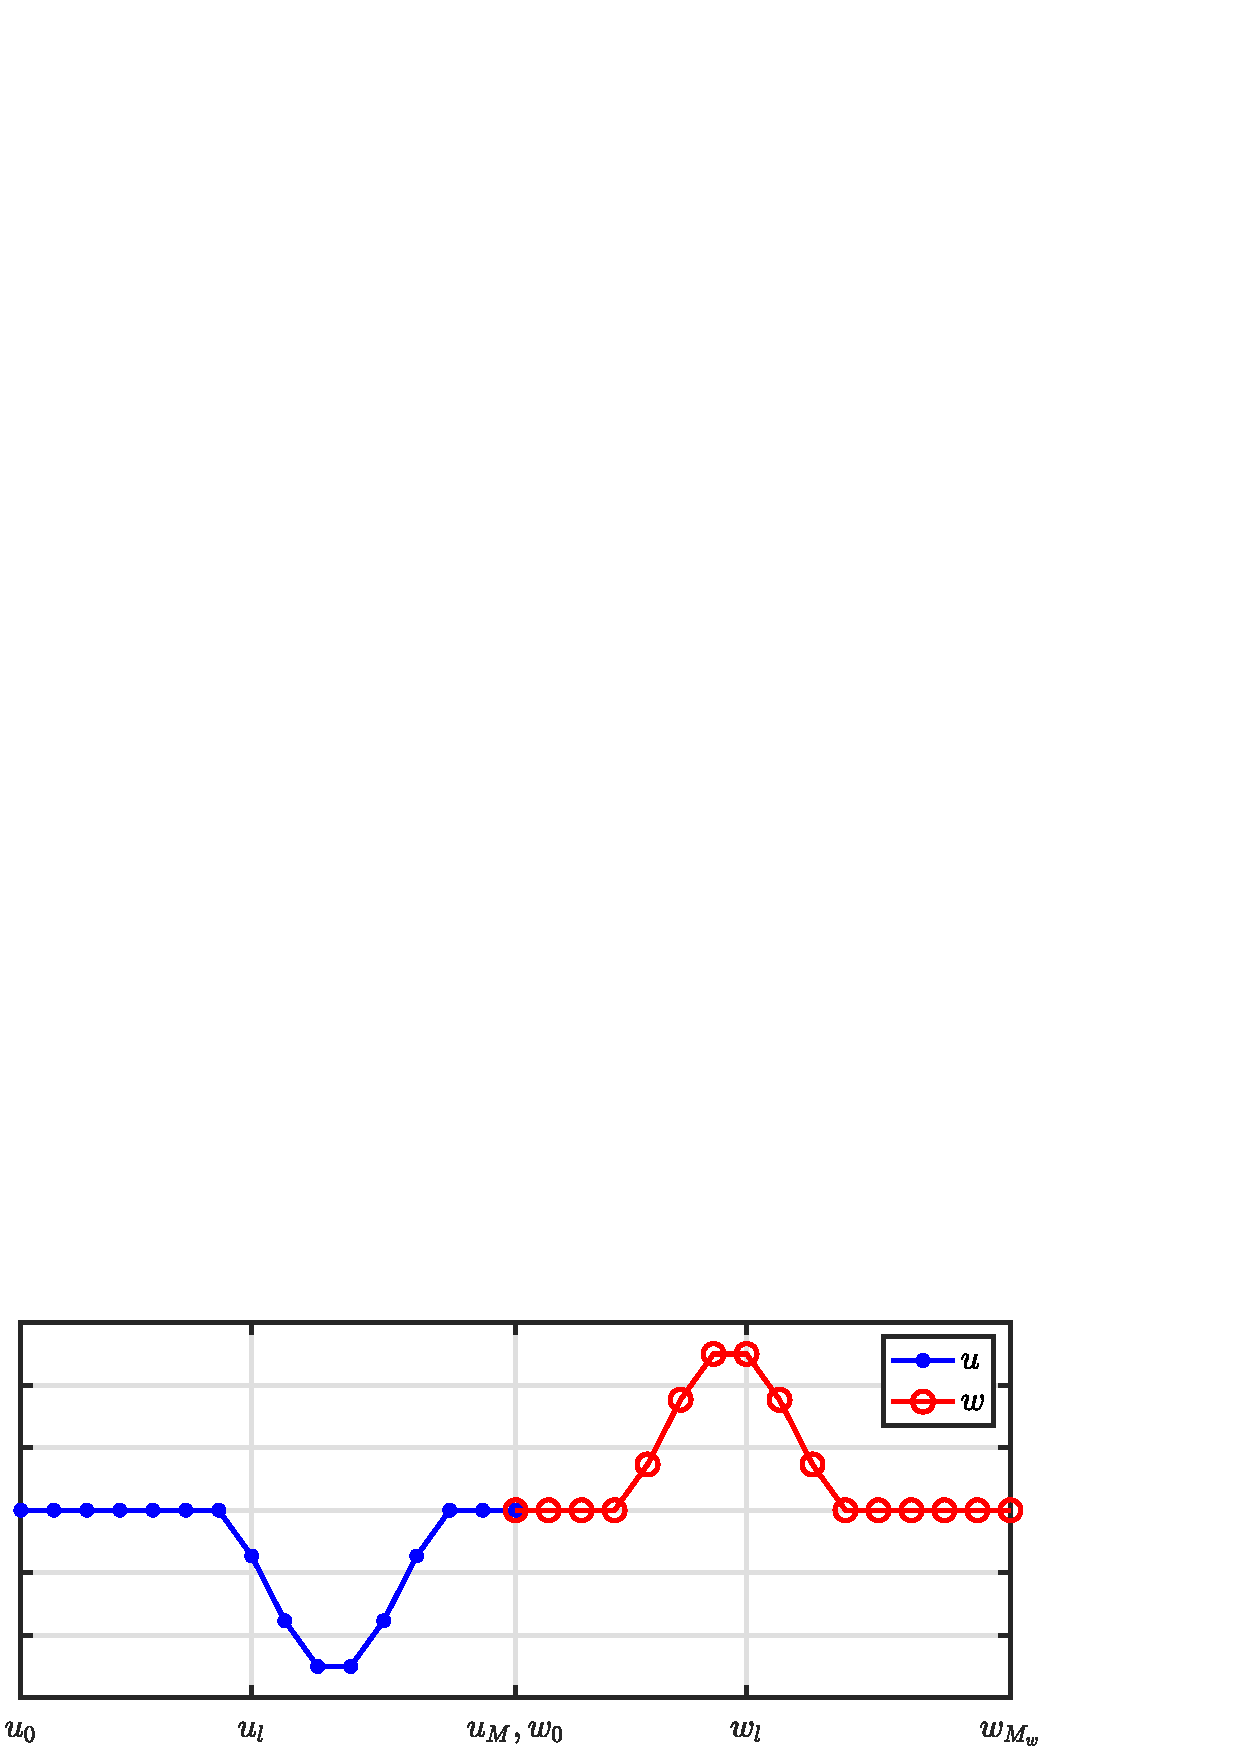
\includegraphics[width=0.8\columnwidth]{twoFreeStrings}}}\\
    \subfloat[]{\label{fig:twoFreeStringsGridMove}{ 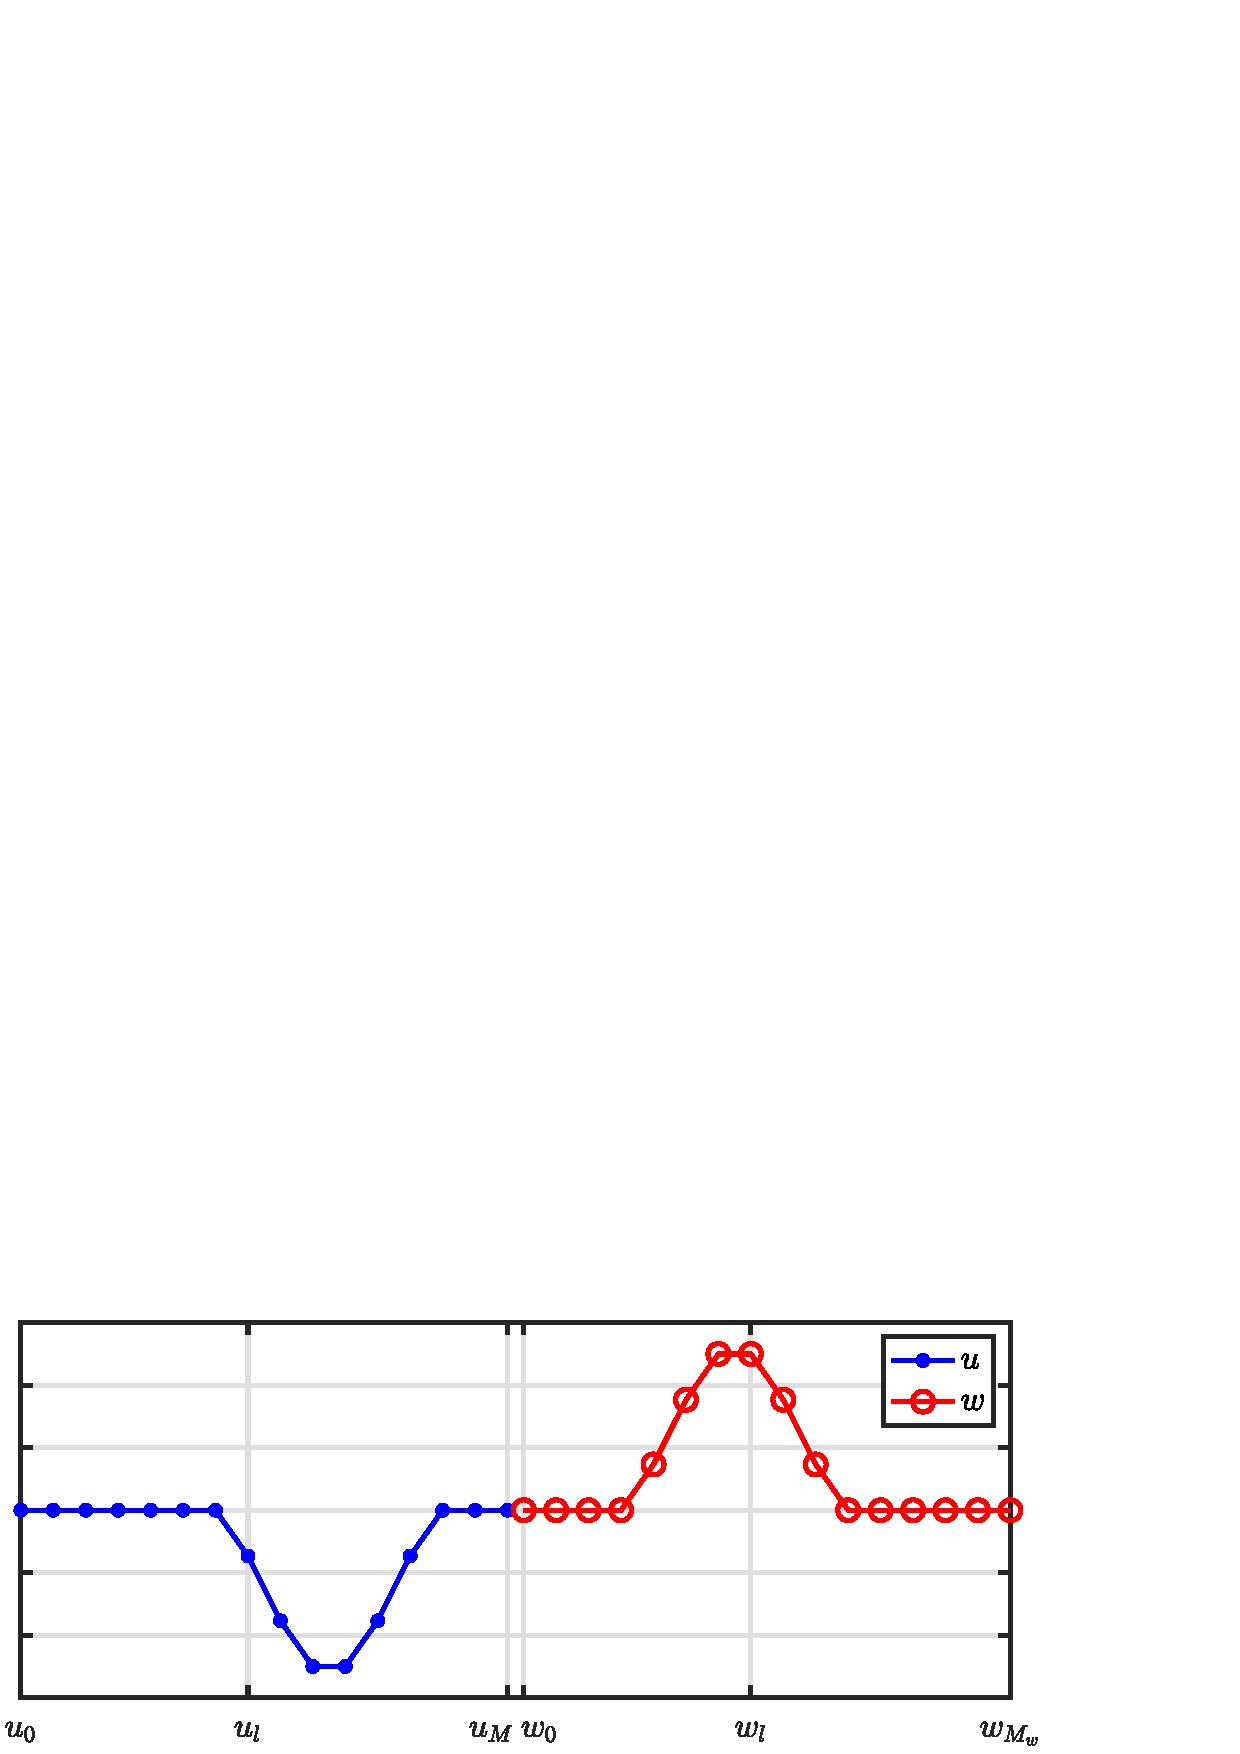
\includegraphics[width=0.8\columnwidth]{twoFreeStringGridMove}}}\\
    \subfloat[]{\label{fig:twoFreeStringsGridZoomed}{ 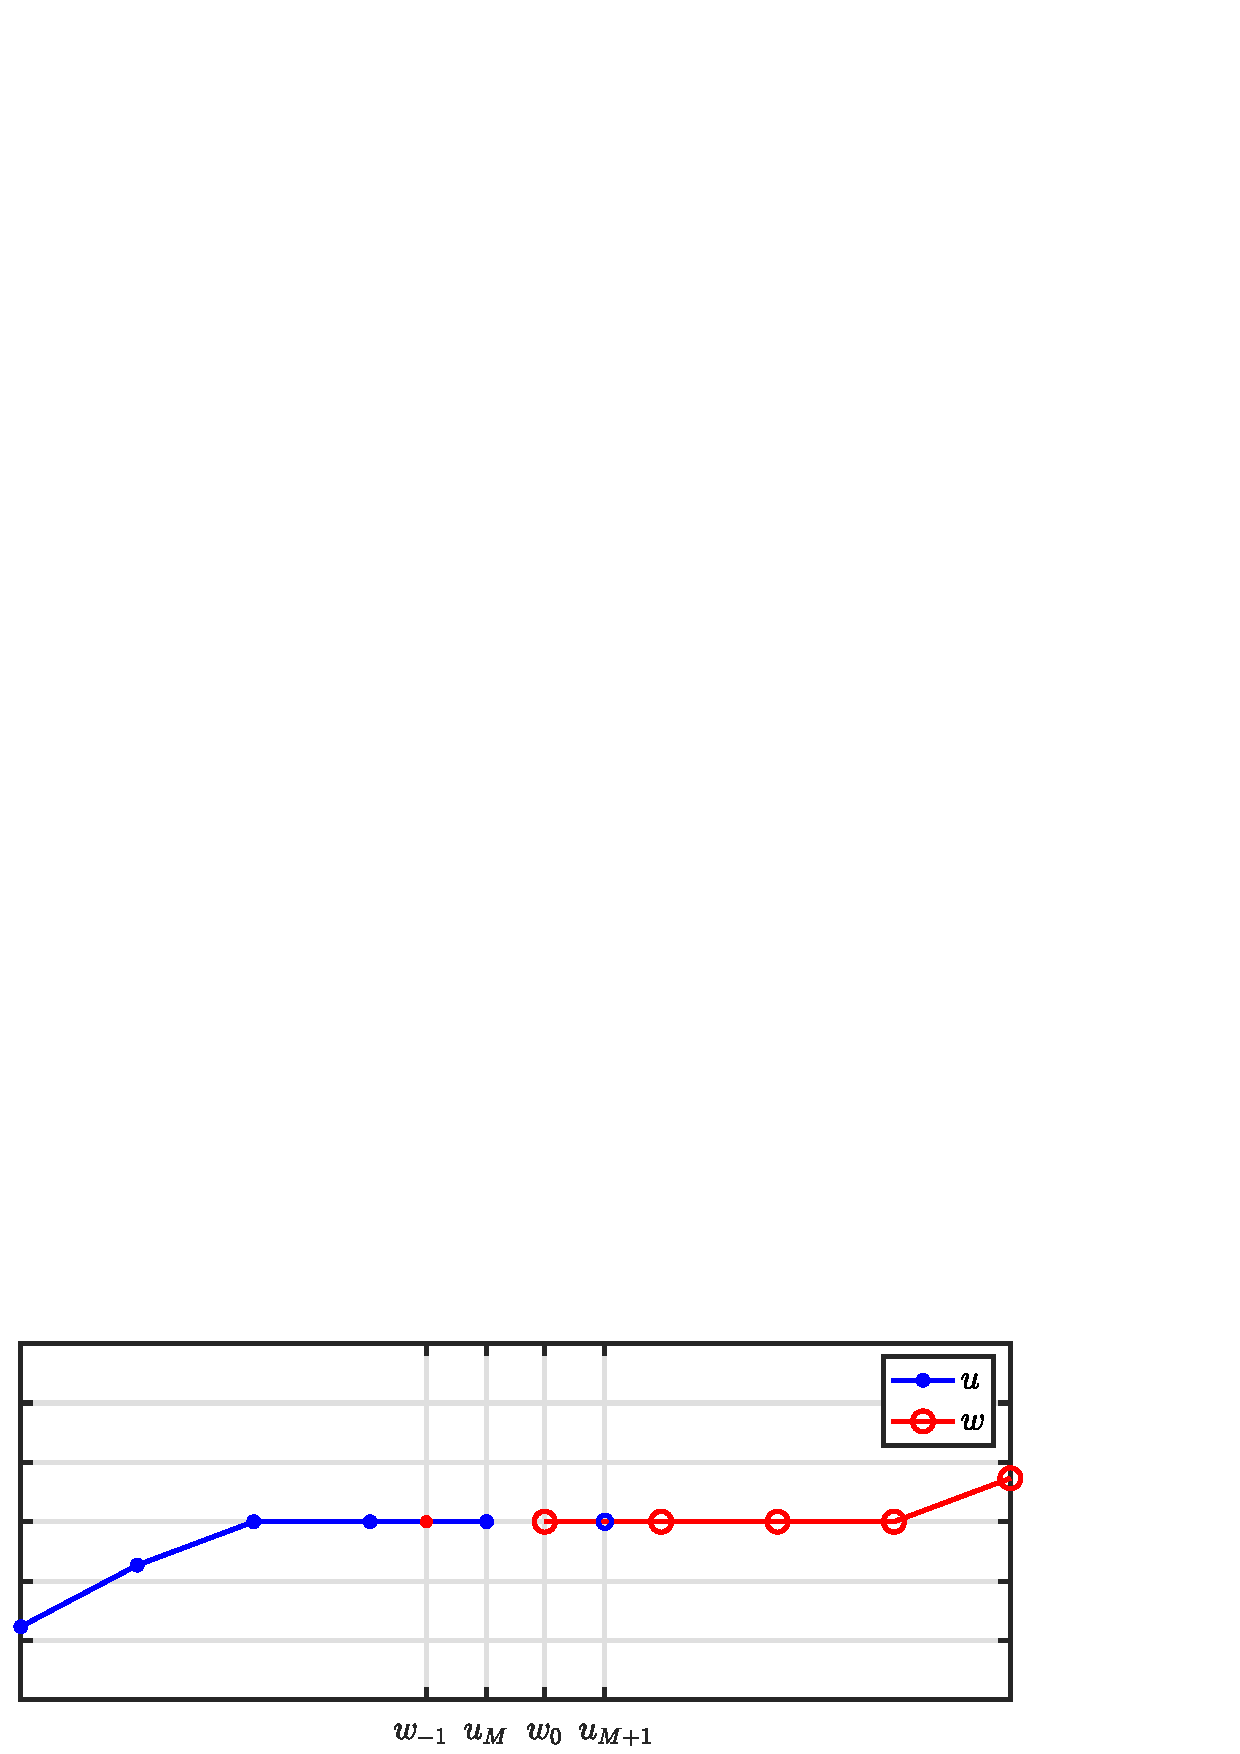
\includegraphics[width=0.8\columnwidth]{twoFreeStringGridMoveZoomed2}}}
    \caption{Illustration of the proposed method. In all figures, the x-axis shows the location (in m) of the respective grid points (fx. $x_{u_l^n}$), but the $x$ and $n$ are omitted for brevity. (a) Locations of the states of two (1D wave) systems connected at the inner boundary ($N = 30$, $x_{u_M}^n = x_{w_0}^n$). (b) When $c$ -- and consequently $h$ -- are decreased and the positions of the grid points change ($N = 30.5$, $x_{u_M}^n \neq x_{w_0}^n$). (c) Figure \ref{fig:twoFreeStringsGridMove} zoomed-in around $x_{u_M}^n$ and $x_{w_0}^n$. The states at the inner boundaries $u_M^n$ and $w_0^n$ are shown together with virtual grid points $u_{M+1}^n$ and $w_{-1}^n$.}
\end{figure}
%
Grid functions $u_l^n$ and $w_l^n$ can then be placed in line with each other with the inner boundaries $u_M^n$ and $w_0^n$ overlapping, i.e., $x_{u_M}^n = x_{w_0}^n$, and the outer boundaries located at $x_{u_0} = 0$ and $x_{w_{M_w}} = L$. The systems can then be connected using a rigid connection
\begin{equation}\label{eq:rigid}
    u_M^n = w_0^n,\quad \forall n.
\end{equation}
To sum up, a grid function with $N = \lfloor L/h\rfloor$ (as per Eq. \eqref{eq:numberOfIntervals}) is divided into two separate subsystems connected at the inner boundary. Even though there is an extra grid point present, the behaviour of the new system should be identical to that of the original system. This will be proved below.

With the above boundary conditions imposed, the following state vectors can be defined:
\begin{equation}
    \begin{aligned}\label{eq:separateStateVectors}
     \mathbf{u}^n &= [u_1^n, \hdots, u_M^n]^T, \\
     \mathbf{w}^n &= [w_0^n, \hdots, w_{M_w-1}^n]^T,
    \end{aligned}
\end{equation}
with $T$ denoting the transpose operation, and have $M$ and $M_{w}$ points respectively. Note that the outer boundaries are excluded as they are 0 at all times. The vector concatenating \eqref{eq:separateStateVectors} is then defined as 
\begin{equation}\label{eq:fullState}
    \U^n = \begin{bmatrix}
        \mathbf{u}^n \\
        \mathbf{w}^n
    \end{bmatrix}.
\end{equation}
Note that the vectors in \eqref{eq:separateStateVectors} and \eqref{eq:fullState} also exist at the next ($n+1$) and previous ($n-1$) time indices. 

Using the above grid functions in the context of the 1D wave equation, system of FDSs can be defined as
\begin{equation}
    \begin{cases}\label{eq:systemHalfStrings}
        \delta_{tt}u_l^n = c^2\delta_{xx}u_l^n + J_u(x_{u_M}^n)F\\
        \delta_{tt}w_l^n = c^2\delta_{xx}w_l^n - J_w(x_{w_0}^n)F
    \end{cases}
\end{equation}
with spreading operators
\begin{equation}
    J_u(x_i) =
    \begin{cases}
        \frac{1}{h}, & l = l_i = \lfloor x_i/h\rfloor\\
        0,& \text{otherwise}
    \end{cases}
    \quad\text{and}\quad
    J_w(x_i) =
    \begin{cases}
        \frac{1}{h}, & l = l_i = \lfloor x_i/h \rfloor - M\\
        0,& \text{otherwise}
    \end{cases}
\end{equation}
applying the effect of the connection \SWcomment[(``connection force", but not really as it isn't in N)] $F$ (in m$^2$/s$^2$) to grid points $u_M^n$ and $w_0^n$ respectively.
%
Expanding the spatial operators in system \eqref{eq:systemHalfStrings} at inner boundaries $u_M^n$ and $w_0^n$, recalling the Neumann condition in  \eqref{eq:halfStringBoundaryCondNeumann} and the definition for the virtual grid points needed for this condition in Eq. \eqref{eq:neumannSolution} yields
\begin{equation}\label{eq:expandedSystem}
    \begin{cases}
        \delta_{tt}u_M^n = \frac{c^2}{h^2}(2u_{M-1}^n-2u_M^n) + \frac{1}{h}F\\
        \delta_{tt}w_0^n = \frac{c^2}{h^2}(2w_1^n-2w_0^n) - \frac{1}{h}F.
    \end{cases}
\end{equation}
Because of Eq. \eqref{eq:rigid}, it is also true that $\delta_{tt}u_M^n = \delta_{tt}w_0^n, \ \forall n$, and $F$ can be calculated by setting the right side of the equations in \eqref{eq:expandedSystem} equal to each other:
\begin{align*}
     \frac{c^2}{h^2}(2u_{M-1}^n-2u_M^n) + \frac{1}{h} F&= 
     \frac{c^2}{h^2}(2w_1^n-2w_0^n) - \frac{1}{h} F\nonumber\\
    % \frac{2}{h}F &= \frac{c^2}{h^2}(2w_1^n - 2u_{M-1}^n)\nonumber\\
    F &= h \frac{c^2}{h^2}(w_1^n - u_{M-1}^n)
\end{align*}
Substituting this into system \eqref{eq:expandedSystem} after expansion of the second-time derivative yields the update of the inner boundaries
% \begin{equation}
\begin{subnumcases}{\!\!\!\!\!\!\!\!\!\!\!\!\!\!\label{eq:resultOneConnectedPoint}}
    u^{n+1}_M = 2u_M^n - u_M^{n-1} + \lambda^2(u_{M-1}^n-2u_M^n+w_1^n)\label{eq:resultUM}\\
    w^{n+1}_0 = 2w_0^n - w_0^{n-1} + \lambda^2(u_{M-1}^n-2w_0^n+w_1^n)\label{eq:resultw0}
\end{subnumcases}
% \end{equation}
which, (again, recalling Eq. \eqref{eq:rigid}) are indeed equivalent expressions for the connected point and is necessary to satisfy the rigid connection. Here, $w_1^n$ in Eq. \eqref{eq:resultUM} acts as virtual grid point $u_{M+1}^n$ and $u_{M-1}^n$ in \eqref{eq:resultw0} as virtual grid point $w_{-1}^n$, essentially connecting the two systems using the state of one in the update of the other.

\subsubsection{Changing the Grid}
The previous section describes the case in which the stability condition is satisfied with equality, i.e, when $1/ck$ is an integer and $x_{u_M}^n = x_{w_0}^n$. The locations of the outer boundaries $x_{u_0}^n$ and $x_{w_{M_w}}^n$ are fixed, i.e.
\begin{equation*}
    x_{u_0}^n = x_{u_0}^0 \quad \text{and}\quad x_{w_{M_w}}^n = x_{w_{M_w}}^0 \quad \forall n.
\end{equation*}
If the wave speed $c$ is then decreased, and consequently the grid spacing $h$ according to $h=ck$, all other points move towards their respective outer boundary (see Figure \ref{fig:twoFreeStringsGridMove}). Calculating $h$ this way allows this method to always satisfy the CFL condition in Eq. \eqref{eq:CFL} with equality, as is the case with the previous iteration described in \ref{sec:iterations}.

% \begin{figure}[h]
% \centerline{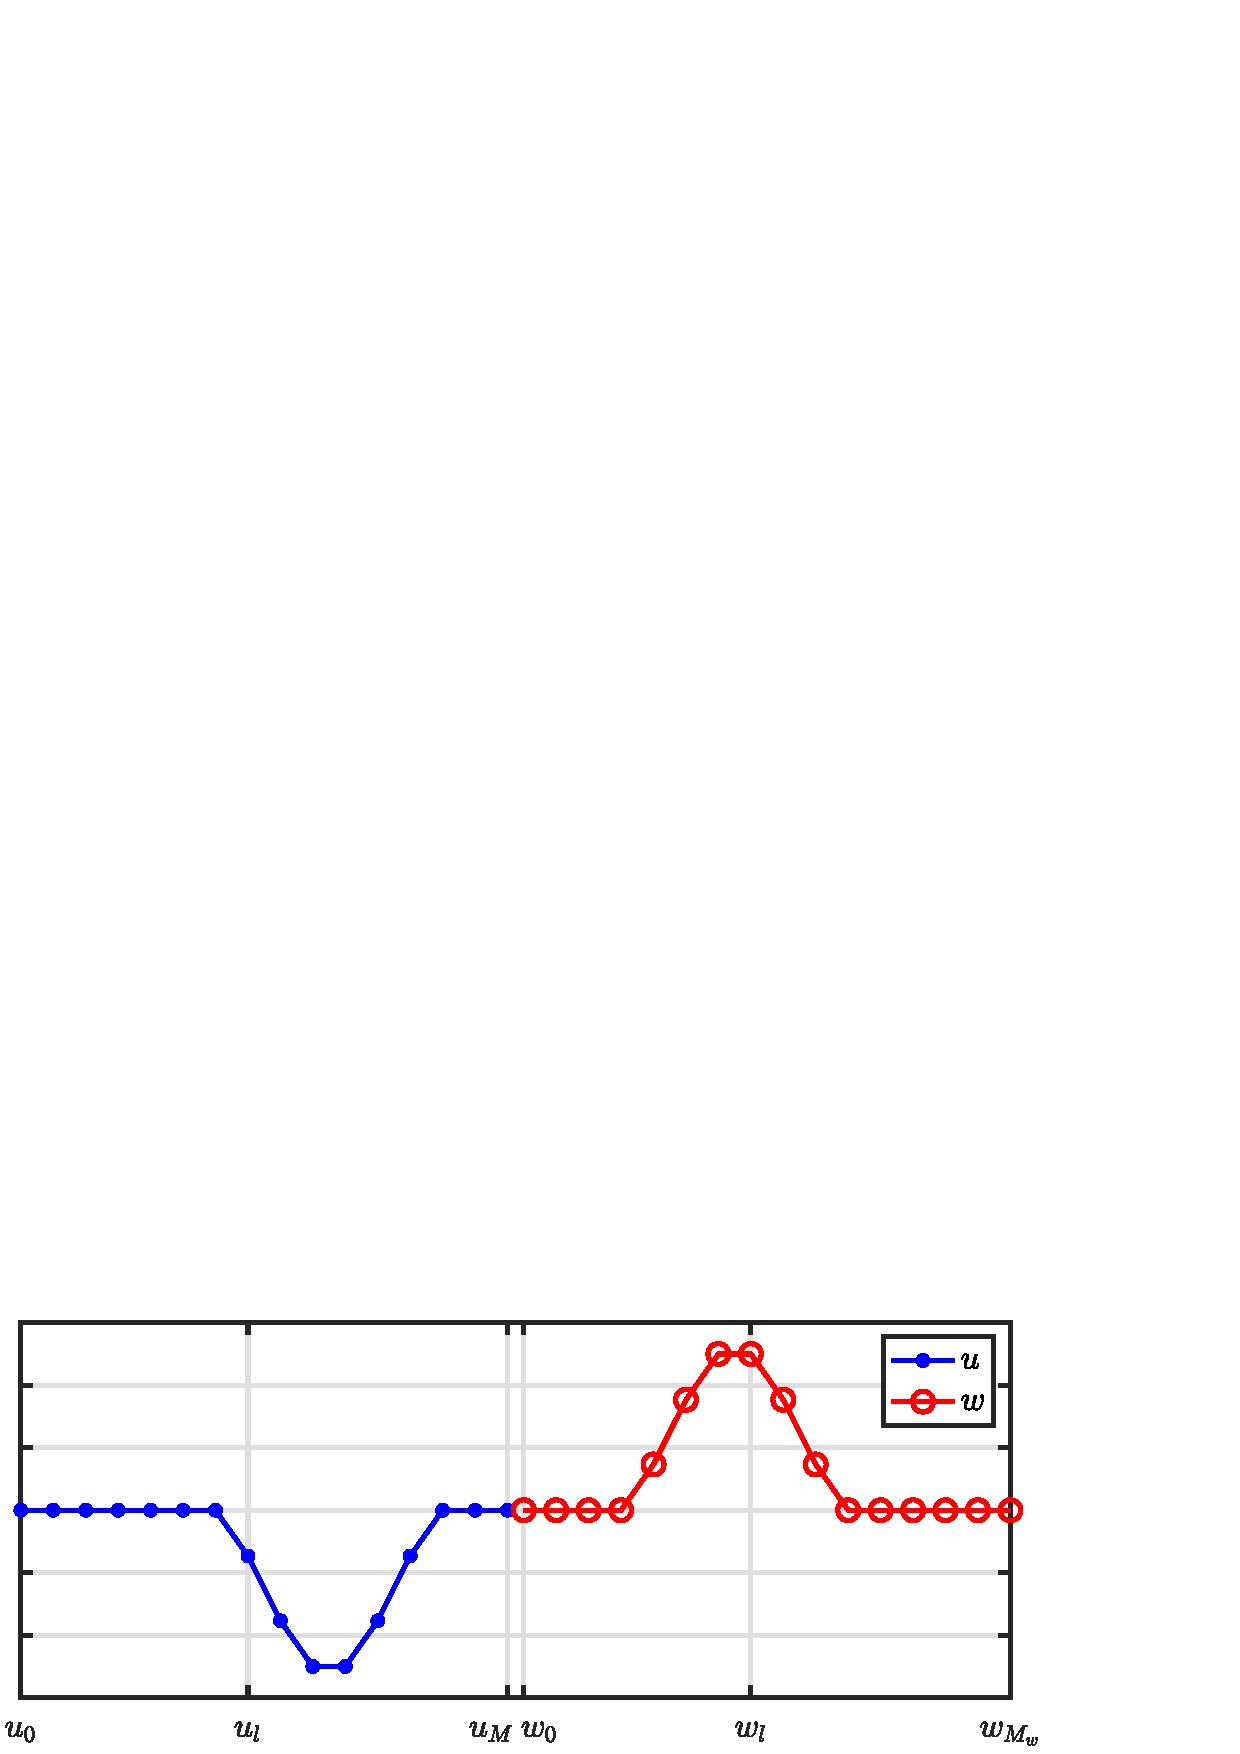
\includegraphics[width=\columnwidth]{twoFreeStringGridMove} }
% \caption{\label{fig:twoFreeStringsGridMove}{When the grid changes ($N = 30.5$). The x-axis shows the location (in m) of the respective grid points (fx. $x_{u_l^n}$), but the $x$ is omitted for clarity.}}
% \end{figure}
%
As mentioned above, the state of $w_l^n$ can be used to calculate virtual grid point needed at the right boundary of $u_l^n$ and vice versa. If the inner boundaries are not overlapping (i.e., $x^n_{u_M} \neq x^n_{w_0}$) a Lagrangian interpolator $I(x_i)$ at location $x_i$ from the left boundary (in m) can be used to calculate the value of this virtual grid point (also see Figure \ref{fig:twoFreeStringsGridZoomed} for reference). The interpolator $I$ is a row-vector the size of $\mathbfcal{U}^n$ (from Eq. \eqref{eq:fullState}) its values depending on what interpolation order is used. In the following, the distance between the inner boundaries normalised with $h$ is defined as
\begin{equation}\label{eq:alphaDef}
    \alpha = \alpha^n = \frac{x^n_{w_0} - x^n_{u_M}}{h}\,,
\end{equation}
and for clarity, $I$ and $\mathbfcal{U}^n$ are indexed by $m$.
Applying the interpolator to $\mathbfcal{U}^n$ yields
\begin{subequations}\label{eq:interpolationGeneral}
    \begin{align}
        u_{M+1}^n &= I^\flip(x^n_{u_{M+1}})\mathbfcal{U}^n% = (1-\alpha)w_1^n + \alpha w_0^n
        \\
        w_{-1}^n &= I(x^n_{w_{-1}})\mathbfcal{U}^n,% = (1-\alpha)u_{M-1}^n + \alpha u_M^n
    \end{align}
\end{subequations}
where $I^\flip$ is a flipped and shifted version of $I$. \SWcomment[$\leftarrow$ further explanation needed here..]
% where
% \begin{equation}
%     \alpha = \frac{x_{w_0} - x_{u_M}}{h},
% \end{equation}
% and grid-point locations $x_{u_{M+1}}$ and $w_{-1}$. Note that when $h$ changes the connected points start to move away from each other.
%
If linear interpolation is used, 
\begin{subequations}\label{eq:linearInterp}
\begin{equation}
    I_1(x_i) = 
    \begin{cases}
        (1-\alpha), & m = m_i \\
        \alpha, & m = m_i + 1\\
        0, & \text{otherwise}
    \end{cases}
\end{equation}
and
\begin{equation}\label{eq:linearFlip}
    I_1^\flip(x_i) = 
    \begin{cases}
        \alpha, & m = m_i^\flip \\
        (1-\alpha), & m = m_i^\flip + 1\\
        0 & \text{otherwise}
    \end{cases}
\end{equation}
\end{subequations}
with $m_i = \lfloor x_i/h\rfloor$ and $m_i^\flip = \lfloor x_i/ h+(1-\alpha) \rfloor$. The shift in the latter is necessary to transform the location to the right indices of $\mathbfcal{U}^n$. \SWcomment[$\leftarrow$ more explanation here] Substituting \eqref{eq:linearInterp} into \eqref{eq:interpolationGeneral} and expanding yields
\begin{subequations}
    \begin{align}
        u_{M+1}^n &= I_1^\flip(x^n_{u_{M+1}})\mathbfcal{U}^n = \alpha w_0^n
        + (1-\alpha)w_1^n,\\
        w_{-1}^n &= I_1(x^n_{w_{-1}})\mathbfcal{U}^n = (1-\alpha)u_{M-1}^n + \alpha u_M^n.
    \end{align}
\end{subequations}
% \begin{figure}[h]
% \centerline{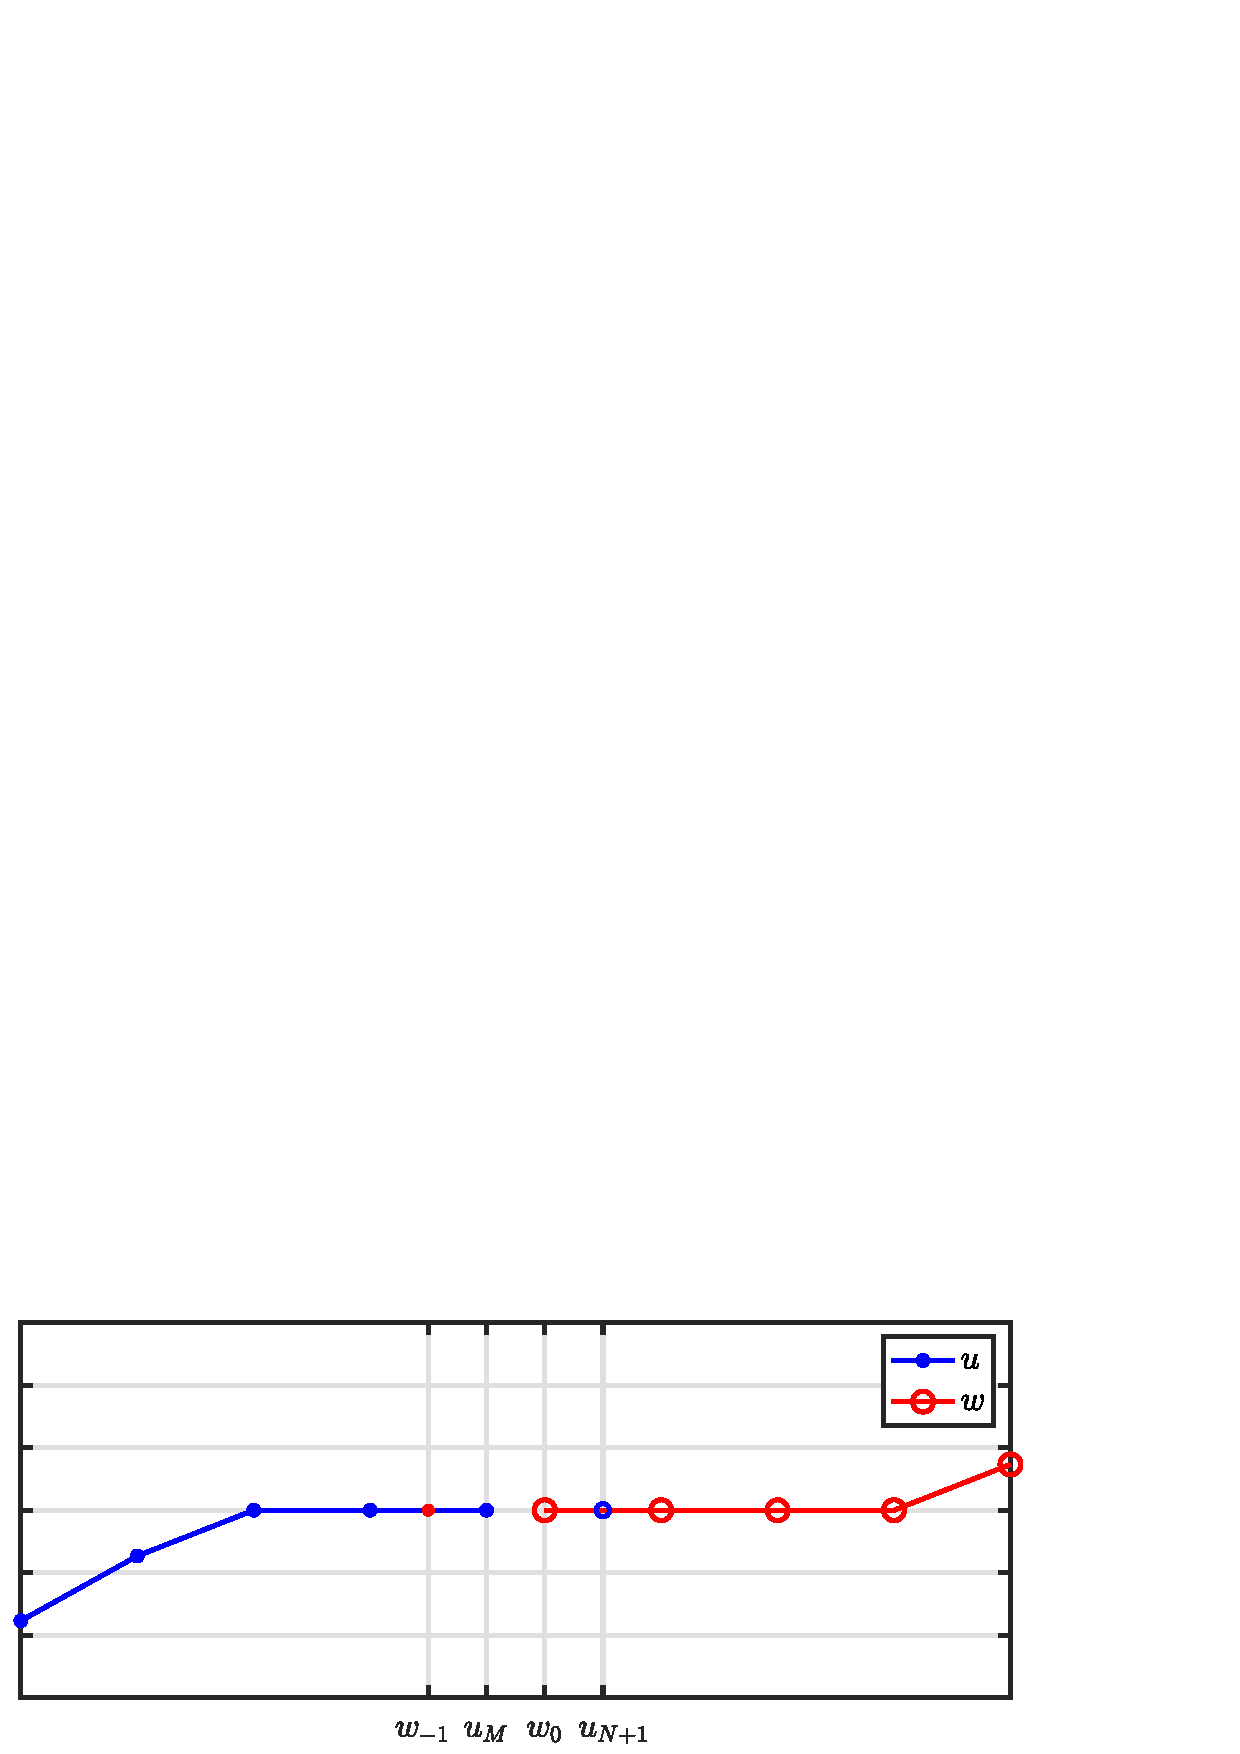
\includegraphics[width=\columnwidth]{twoFreeStringGridMoveZoomed} }
% \caption{\label{fig:twoFreeStringsGridZoomed}{When the grid changes (zoomed). The states at the inner boundaries $u_M$ and $w_0$ are shown together with virtual grid points $u_{M+1}$ and $w_{-1}$.}}
% \end{figure}
%
Using $I_1$, analysis of the output shows that the expected fundamental frequency $f_0$ is slightly higher when interpolation needs to happen than the one expected when using Eq. \eqref{eq:fundamentalFreq}. Furthermore, modes higher than $f_\text{s} / 4$ would follow an odd pattern up when decreasing the wavespeed, opposite of what is expected. \SWcomment[$\leftarrow$ didn't know where (or whether) to include this.]

One could extend the range of interpolation by one point to each side, using a cubic Lagrange interpolator instead. Though this would require $w_{-1}^n$ to calculate $u_{M+1}^n$ and vice versa, it is possible to solve this by treating the interpolation equations as a system of linear equations. Analysis of this method, though yielding a correct $f_0$ at all times, shows similar behaviour to the linear interpolation, with odd behaviour regarding to modes higher than $f_\text{s}/4$.

Much better behaviour is observed when points of both $u_l^n$ and $w_l^n$ are used to calculate the values of the virtual grid points. This means to also use $u_M^n$ to calculate $u_{M+1}^n$ and $w_0^n$ for $w_{-1}^n$. Now, the locations of the grid points used in the interpolation are not equidistant and a custom Lagrangian interpolator needs to be created. The lowest order interpolator that can be used here is the quadratic interpolator $I_2$
\begin{equation}
    I_2(x_i) =
    \begin{cases}
        -(\alpha-1)/(\alpha + 1), & m = m_i-1\\
        1 & m = m_i\\
        (\alpha-1)/(\alpha + 1), & m = m_i+1\\
        0, & \text{otherwise}
    \end{cases}
\end{equation}
(the flipped version $I_2^\flip$ defined similarly to \eqref{eq:linearFlip}) and when applied to Eq. \eqref{eq:fullState} yields
\begin{subequations}\label{eq:connectionInterpol}
\begin{align}
    &\begin{aligned}\label{eq:calcUMP1}
        u_{M+1}^n = I_2^\flip(x^n_{u_{M+1}})\mathbfcal{U}^n = \frac{\alpha - 1}{\alpha + 1}u_{M}^n + w_0^n - \frac{\alpha - 1}{\alpha + 1}w_1^n
    \end{aligned}\\
    &\ \ \begin{aligned}\label{eq:calcWM1}
        w_{-1}^n = I_2(x^n_{w_{-1}})\mathbfcal{U}^n
        =-\frac{\alpha - 1}{\alpha + 1}u_{M-1}^n + u_{M}^n+ \frac{\alpha - 1}{\alpha + 1}w_{0}^n.
    \end{aligned}
\end{align}
\end{subequations}
% where
% \begin{equation}\small
% \begin{gathered}\label{eq:interpolationCoeffs}
%     \alpha_\text{I} = \frac{\alpha(\alpha - 1)(\alpha - 2)}{-6}, \quad \beta_\text{I} = \frac{(\alpha - 1)(\alpha + 1)(\alpha - 2)}{2},\\
%     \gamma_\text{I} = \frac{\alpha(\alpha + 1)(\alpha - 2)}{-2}, \quad \text{and} \quad\delta_\text{I} = \frac{\alpha(\alpha + 1)(\alpha - 1)}{6}\,.
% \end{gathered}
% \end{equation}
% Treating \eqref{eq:connectionInterpol} as a system of linear equations, the virtual grid points $u_{M+1}^n$ and $w_{-1}^n$ can be solved for using
% \begin{equation}\label{eq:linSystSolution}
%     \begin{bmatrix}
%     u_{M+1}^n \\
%     w_{-1}^n
%     \end{bmatrix}
%     =
%     \mathbfcal{A}\begin{bmatrix}
%     \alpha_\text{I} w_2^n+ \beta_\text{I}w_1^n + \gamma_\text{I}w_0^n \\
%     \alpha_\text{I} u_{M-2}^n + \beta_\text{I}u_{M-1}^n + \gamma_\text{I} u_{M}^n
%     \end{bmatrix},
% \end{equation}
% where
% \begin{equation}\label{eq:Amat}
%     \mathbfcal{A} = \begin{bmatrix}
%          1 & -\delta_\text{I} \\
%          -\delta_\text{I} & 1
%     \end{bmatrix}^{-1}.\nonumber
% \end{equation}
% where
% \begin{equation}\nonumber
%     \mathbfcal{A} = \begin{bmatrix}
%          1 & -\delta_\text{I} \\
%          -\delta_\text{I} & 1
%     \end{bmatrix},
% \end{equation}
% and
% \begin{equation}\nonumber
%     \mathbf{v} = \begin{bmatrix}
%     \alpha_\text{I} w_2^n+ \beta\text{I}w_1^n + \gamma\text{I}w_0^n \\
%     \alpha_\text{I} u_{M-2}^n + \beta\text{I}u_{M-1}^n + \gamma u_{M}^n
%     \end{bmatrix}.
% \end{equation}
As will be shown in the Results section, quadratic interpolation yields the expected fundamental frequency at all times. One can show that when $N$ is an integer, and thus $\alpha = 0$, Eqs. \eqref{eq:calcUMP1} and \eqref{eq:calcWM1} can be substituted as $w_1^n$ and $u_{M-1}^n$ into Eqs. \eqref{eq:resultUM} and \eqref{eq:resultw0} respectively (as these acted as virtual grid points $u_{M+1}^n$ and $w_{-1}^n$). Then recalling Eq. \eqref{eq:rigid} it can be seen that the system is reduced to \eqref{eq:resultOneConnectedPoint}. % also when interpolation needs to happen.

\subsubsection{Adding and removing Grid Points}
When $c$, and consequently $h$, is decreased and the inner boundary points surpass the virtual points (i.e. $x_{u_M}^n \leq x_{w_{-1}}^n$ and $x_{w_0}^n \geq x_{u_{M+1}}^n$) and $\lfloor N^n\rfloor > \lfloor N^{n-1}\rfloor$, a point is added to the right boundary of $u_l^n$ and the left boundary of $w_l^n$ (for both time indices $n$ and $n-1$) in an alternating fashion: 
\begin{equation}\label{eq:addingPoint}
        \begin{cases}\mathbf{u}^n = [\mathbf{u}^n, I_3\mathbf{v}^n]^T & \text{if $\lfloor N^n\rfloor $ is odd},\\
        \mathbf{w}^n = [I_3^\flip\mathbf{v}^n, \mathbf{w}^n]^T & \text{if $\lfloor N^n\rfloor$ is even},
        \end{cases}
\end{equation}
where 
\begin{align*}
\mathbf{v}^n = [u_{M-1}^n, u_M^n, w_0^n, w_1^n]^T,% \quad\text{and}\\
%     \mathbf{v}_\star^n &= [w_1^n, w_0^n, u_M^n, u_{M-1}^n],
\end{align*}
and cubic Lagrangian interpolator
\begin{equation}\label{eq:customIp}
    I_3 = \begin{bmatrix} -\frac{\alpha'(\alpha'+1)}{(\alpha'+2)(\alpha'+3)} &\frac{2\alpha'}{\alpha'+2} &\frac{2}{\alpha'+2} 
    &-\frac{2\alpha'}{(\alpha'+3)(\alpha'+2)}
    \end{bmatrix},
\end{equation}
with
\begin{equation*}
    \alpha' = \frac{x_{w_0}^n - (x_{u_M}^n + h)}{h}\ .
\end{equation*}
See Figure \ref{fig:addingPoint}.
% Note that this operation is done for both time indices $n$ and $n-1$.

\begin{figure}[h]
    \centering
%% \reprintcolumnwidth is the same in preprint and reprint for
%% ease of use for authors:
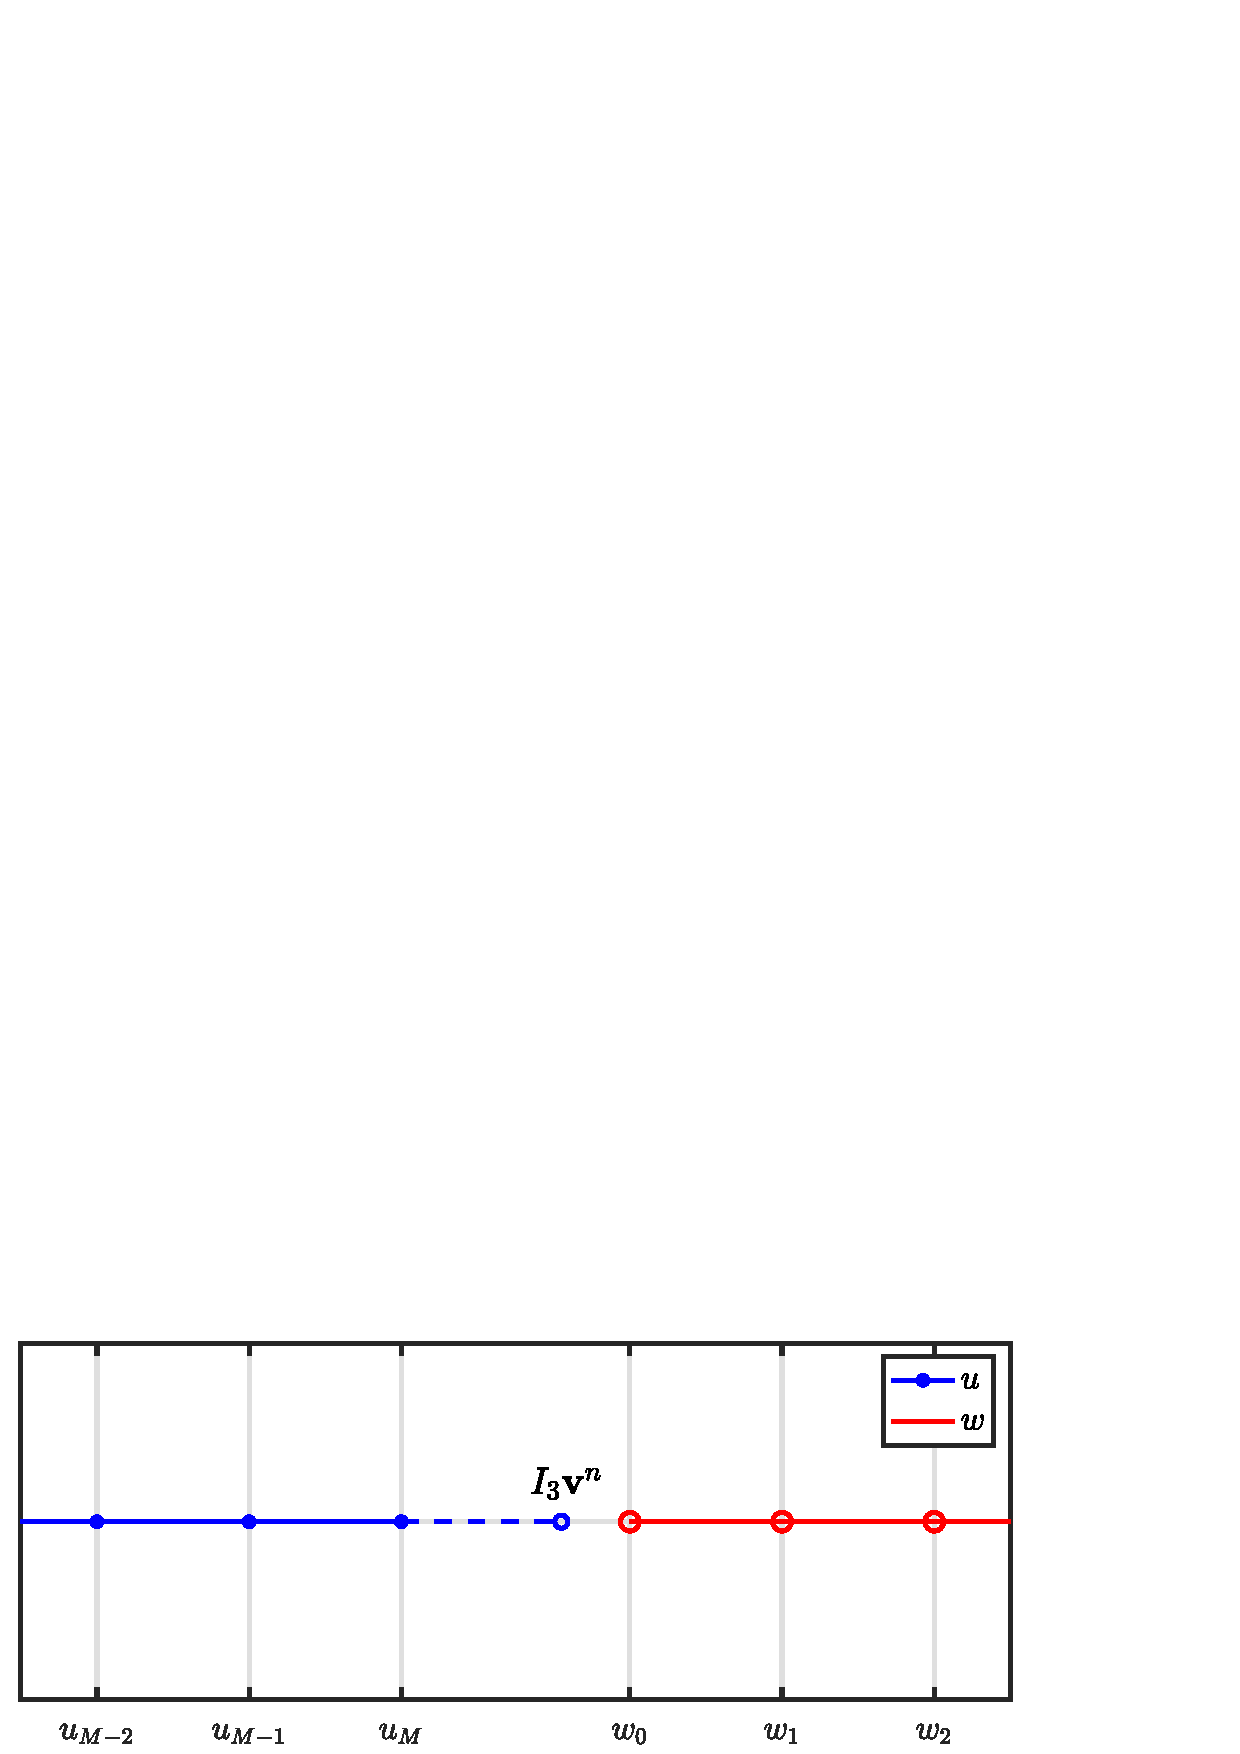
\includegraphics[width=0.8\columnwidth]{addingGridPoint4}
\caption{\label{fig:addingPoint}{The moment when a point is added to $\mathbf{u}$ at location $x_{u_M} + h$ in Eq. \eqref{eq:addingPoint}. This figure shows an extreme case where this location is far from $x_{w_0}$, i.e., $\alpha' \not\approx 0$ in Eq. \eqref{eq:customIp}.}}
\end{figure} 

Except in the case of extremely quick parameter variations, $\alpha'$ in Eq. \eqref{eq:customIp} is expected to be close to zero, i.e., $x_{u_M}^n + h \approx x_{w_0}^n$, meaning that $I_3 \approx [0, 0, 1, 0]$. This makes sense by looking at Figure \ref{fig:twoFreeStringsGridZoomed}, as exactly when the boundary points $u_M^n$ and $w_0^n$ surpass the virtual points $w_{-1}^n$ and $u_{M+1}^n$, these are going to be close to overlapping.

Removing grid points happens when $c$, and consequently $h$, is increased and $x_{u_M}^n \geq x_{w_0}^n$ (or $\lfloor N^n\rfloor < \lfloor N^{n-1}\rfloor$). Compared to adding grid points, removing these is slightly more straightforward as points are simply removed from $\mathbf{u}$ and $\mathbf{w}$ (again for both $n$ and $n-1$) in an alternating fashion
\begin{equation}\label{eq:removingPoint}
\begin{cases}
    \mathbf{u}^n = [u_0^n, u_1^n ..., u_{M-1}^n]^T & \text{if $N^n$ is even}, \\
     \mathbf{w}^n = [w_1^n, w_2^n ..., w_{M_w}^n]^T & \text{if $N^n$ is odd}.
    \end{cases}
\end{equation}

A problem that arises from simply removing a grid points, is that it is possible that $u_M^n \not\approx w_0^n$ at the time of removal. As $x_{u_M}^n \approx x_{w_0}^n$ at the time of removal (except for extremely quick parameter variations), this violates the rigid connection in \eqref{eq:rigid} and causes audible artefacts. A method of displacement correction is proposed that decreases the relative displacement of the inner boundaries the closer their grid-locations are together, i.e., the closer $\alpha$ in \eqref{eq:alphaDef} is to 0:
\begin{equation}\label{eq:dispCorr}
    \begin{aligned}
    u_M^n := u_M^n +\beta (w_0^n - u_M^n),\\
    w_0^n := w_0^n - \beta  (w_0^n - u_M^n),
    \end{aligned}
\end{equation}
with
\begin{equation}\label{eq:betaDef}
    \beta(\epsilon) = \frac{(1-\alpha)^\epsilon}{2}
\end{equation}
where $\epsilon \geq 1$ is a tunable parameter. A lower $\epsilon$ decreases the chance of artifacts but will have a greater low-passing effect on the system. For low-speed changes, using $\sim 1000$ samples for removing one grid point, $\epsilon \approx 30$ ensures that $u_M^n \approx w_0^n$ and already suffices to remove artefacts arising from point removal.

Until now, only adding and removing points in the center of the system has been considered. This location could be moved anywhere along the grid, the limit being one point from the boundary. Furthermore, one does not have to add and remove points from $\mathbf{u}$ and $\mathbf{w}$ in an alternating fashion as in \eqref{eq:addingPoint}, but can just add and remove from (fx.) $\mathbf{u}$ leaving $\mathbf{w}$ the same size throughout the simulation. In the extreme case where $M = \lfloor N\rfloor - 1$ and $M_w = 1$ (leaving $\mathbf{w}$ with only one moving grid point, $w_0^n$) the method still works.
% 
% \SWcomment[The following applies to odd-ordered Lagrange interpolators $\rightarrow$] The location at where points are added and removed greatly influences the behaviour of the system, especially in the higher frequencies (see Section \ref{sec:results}). The best behaviour is obtained when the location is as close to a boundary as possible. 

\subsection{Summary}
Here, Section \ref{sec:proposedMethod} is summarised and describes the final version of the proposed method.

The method subdivides a grid function with $N+1$ grid points into two grid functions $u_l^n$ and $w_l^n$ with $M+1$ and $M_w+1$ grid points respectively. Knowing that $\lambda=1\ \forall n$, Eq. \eqref{eq:updateEq}, written for both grid functions, becomes 
\begin{subequations}\label{eq:uwUpdates}
    \begin{align}
        u_l^{n+1} &= u_{l+1}^n + u_{l-1}^n - u_l^{n-1},\label{eq:uUpdate}\\
        w_l^{n+1} &= w_{l+1}^n + w_{l-1}^n - w_l^{n-1}\label{eq:wUpdate},
    \end{align}
\end{subequations}
%
Due to the Dirichlet boundary condition in \eqref{eq:discreteDirichlet} imposed on the outer boundaries of the system, $u_0^n$ and $w_{M_w}^n$ are $0$ at all times and are not included in the calculation. The range of calculation for Eq. \eqref{eq:uUpdate} and \eqref{eq:wUpdate} then become $l = [1, \hdots, M]$ and $l = [0, \hdots, M_w - 1]$ respectively. 

The inner boundaries are calculated using
\begin{subequations}
    \begin{align}
        u_M^{n+1} &= u_{M+1}^n + u_{M-1}^n - u_M^{n-1},\\
        w_0^{n+1} &= w_{-1}^n + w_{2}^n - w_0^{n-1}.
    \end{align}
\end{subequations}
%
where virtual grid points $u_{M+1}^n$ and $w_{-1}^n$ can be calculated using Eq. \eqref{eq:connectionInterpol}.

Then, when $\lfloor N^n \rfloor > \lfloor N^{n-1} \rfloor$ a point is added to $\mathbf{u}^n$ and $\mathbf{u}^{n-1}$ (or $\mathbf{w}^n$ and $\mathbf{w}^{n-1}$) using Eq. \eqref{eq:addingPoint}, and when $\lfloor N^n \rfloor <\lfloor N^{n-1} \rfloor$ a point is removed from the same vectors using Eq. \eqref{eq:removingPoint}. In order to prevent audible artefacts when increasing $c$ (and thus decreasing $N$), the displacement correction in \eqref{eq:dispCorr} is proposed to ensure that the inner boundaries have a similar displacement when one of them is removed.

Finally, using $\mathbfcal{U}$ from Eq. \eqref{eq:fullState} the total system can then be compactly written in matrix form as
\begin{equation}\label{eq:totalSystem}
    \mathbfcal{U}^{n+1} = 
    \mathbf{B} 
    \mathbfcal{U}^n
    - \mathbfcal{U}^{n-1}
\end{equation}
with $\lfloor N\rfloor \times \lfloor N\rfloor$ matrix
\begin{equation}\label{eq:bMat}\small
    \mathbf{B} = \begin{bmatrix}[cccc|cccc]
        & \ddots  &\ddots & & & & 0 & \\
          & 1 & 0 & 1 & & & & \\
         & & 1 & \frac{\alpha - 1}{\alpha + 1} - \beta  & 1 + \beta & -\frac{\alpha - 1}{\alpha + 1} & \\ \cline{2-7}
         & & -\frac{\alpha - 1}{\alpha + 1} & 1 + \beta & \frac{\alpha - 1}{\alpha + 1} - \beta  & 1 & & \\
            & & & &1 & 0 & 1  \\
            & 0 & &  &  &\ddots & \ddots &
       \end{bmatrix}
\end{equation}
%
% \begin{equation}\small
%     \mathbf{B} = \begin{bmatrix}[ccccccc|cc]
%     & &\ddots &\ddots & \ddots  & & \mathbf{0} & & \\
%      & & &1 & 0 & 1 & & \mathbf{0} & \\
%      & & &  & 1 & 0 & 1 & & \\
%      & &\mathbf{0} &  & \mathbfcal{A}_{1, 2}\alpha_\text{I} &\mathbfcal{A}_{1, 2}\beta_\text{I} + 1 &\mathbfcal{A}_{1, 2}\gamma_\text{I} & \mathbfcal{A}_{1, 1}(\gamma_\text{I}-\alpha_\text{I})& \\ \cline{2-8}
%      & & \mathbf{0} & &\mathbfcal{A}_{2, 2}\alpha_\text{I} &\mathbfcal{A}_{2, 2}\beta_\text{I}&\mathbfcal{A}_{2, 2}\gamma_\text{I} & \mathbfcal{A}_{2,1}(\gamma_\text{I} - \alpha_\text{I}) & 
%     \end{bmatrix}
% \end{equation}
%
Notice that when $\alpha$ approaches $1$, $\mathbf{B}$ will reduce to a matrix with ones on the diagonals next to the main diagonal and zeros elsewhere, which translates directly to the usual situation in Eq. \eqref{eq:updateEq} with $N = M + M_w + 1$. 

\subsection{Implementation}
When implementing this method, it is important not to change the grid as the scheme is calculated. I.e., the same $\alpha$ and $\beta$ need to be used to calculate $u^n_l$ and $w^n_l$ at time index $n$ for all $l$.

% \begin{algorithmic}[ht]
% \vspace{1em}
% \fbox{\parbox{0.8\linewidth}{
% \setstretch{1.5}
% \While{application is running}
% \State Wavespeed $c$ is changed
% \If{$\lfloor N^n\rfloor > \lfloor N^{n-1} \rfloor$}
%   \State Add point (Eq. \eqref{eq:addingPoint})
% \ElsIf{$\lfloor N^n\rfloor < \lfloor N^{n-1} \rfloor$}
%   \State Remove point (Eq. \eqref{eq:removingPoint})
% \EndIf
%     \State Calc. $\alpha$ and $\beta$ (Eqs. \eqref{eq:alphaDef} and \eqref{eq:betaDef})
%     \State Calc. scheme (Eq. \eqref{eq:totalSystem})
%     \State Retrieve output
%     \State Update FDS States
% \EndWhile}}
% % \caption{Pseudo code showing the order of calculation \label{alg:calcOrder}}
% \end{algorithmic}

\SWcomment[going to include some pseudocode here to rather than the list below]
\begin{itemize}
    \item Wavespeed is changed
    \item Check whether $\lfloor N^n\rfloor \neq \lfloor N^{n-1} \rfloor$
    \begin{itemize}
        \item If so add/remove point using \eqref{eq:addingPoint} or \eqref{eq:removingPoint}
    \end{itemize}
    \item Calculate $\alpha$ and $\beta$ in \eqref{eq:bMat} using \eqref{eq:alphaDef} and \eqref{eq:betaDef}.
    \item Calculate scheme \eqref{eq:totalSystem}
    \item Retrieve output
    \item Update states
\end{itemize}
